\documentclass[]{scrartcl}
\usepackage[utf8]{inputenc}
\usepackage[T1]{fontenc}
\usepackage[T2A]{fontenc}
\usepackage[finnish]{babel}
\usepackage{linguex} 
\usepackage{longtable} 
\usepackage{booktabs}
\usepackage{amsthm}
\usepackage{placeins}
\usepackage{graphicx}
\newtheorem{maar}{Määritelmä}
\usepackage{fixltx2e} % provides \textsubscript
\usepackage{textcomp} % provides \textsubscript
\usepackage{hyperref}
\usepackage{xcolor}

\providecommand{\tightlist}{%
  \setlength{\itemsep}{0pt}\setlength{\parskip}{0pt}}

\hypersetup{
    colorlinks,
    linkcolor={red!50!black},
    citecolor={blue!50!black},
    urlcolor={blue!80!black}
}
\author{Juho Härme}
\title{Morfologia-kurssin luentomateriaaleja}
\date{\today}
\begin{document}
\maketitle
\tableofcontents
\newpage



\section{Luento 15: Aika ja aspekti kieliopillisina
kategorioina}\label{luento-15-aika-ja-aspekti-kieliopillisina-kategorioina}

\begin{itemize}
\tightlist
\item
  \href{https://mustikka.uta.fi/~juho_harme/morfologia/\#tästä-kurssista}{Takaisin
  sivun ylälaitaan}
\item
  \href{http://mustikka.uta.fi/~juho_harme/morfologia/materiaalit/luento15.pdf}{Lataa
  PDF}
\item
  \href{http://mustikka.uta.fi/~juho_harme/morfologia/presentations/luento15.html}{Tutki
  luentokalvoja}
\item
  \href{http://mustikka.uta.fi/~juho_harme/morfologia/tehtavat/luento15.pdf}{Tutki
  tuntitehtäviä}
\end{itemize}

Aika on varsin poikkitieteellinen käsite. Se on merkittävä niin
filosofisessa, psykologisessa, lingvistisessä kuin fysikaalisessakin
mielessä. On luonnollista, että ajan ilmaiseminen kielessä on yksi
keskeisimmistä ja tärkeimmistä kysymyksistä, joita niin kielenoppija
kuin -tutkija joutuu pohtimaan. Menemättä sen syvempiin filosofisiin
pohdintoihin, todettakoon käytännön tasolla, että ajan ja ajallisten
suhteiden ilmaisuun voidaan luonnollisissa kielissä käyttää ainakin
\emph{verbien aikamuotoja}, \emph{aspektia}, \emph{adverbeja} sekä
esimerkiksi kiinan kielessä olevia \emph{temporaalipartikkeleita} (Klein
{[}1994{]} 1999, 143). Tällä ja seuraavilla kahdella luennollolla
keskitymme kahteen ensiksi mainittuun kieliopilliseen kategoriaan:
aikamuotoihin eli tempukseen (категория времени) sekä aspektiin
(категория вида).

\subsection{Aikamuodot venäjässä}\label{aikamuodot-venuxe4juxe4ssuxe4}

Aikaa ja aspektuaalisuutta paljon tutkineen kielitieteilijän A.V.
Bondarkon (2005: 261) mukaan venäjässä käytössä olevat aikamuodot
(aikakategorian arvot) on perinteisimmän tulkinnan mukaisesti jaettu
seuraavan taulukon kuvaamalla tavalla:

\begin{longtable}[c]{@{}lll@{}}
\toprule
Aika & muoto1 & muoto 2\tabularnewline
\midrule
\endhead
Mennyt (preteriti) & прошедшее несовершенное & прошедшее
совершенное\tabularnewline
Nykyhetki (preesens) & настоящее несовершенное & -\tabularnewline
Tuleva (futuuri) & будущее несовершенное & будущее
совершенное\tabularnewline
\bottomrule
\end{longtable}

Taulukko kiinnittää huomion siihen, että aikaa ilmaistaessa
aikamuotokategoria ja aspektikategoria toimivat venäjässä yhteistyössä:
ei oikeastaan ole mahdollista puhua aikamuodoista puhumatta myös
aspektista. On tähdennettävä, että esitetyt muodot koskevat ainoastaan
\emph{indikatiivin} tapaluokkaa (изъявительное наклонение). Tutkitaan
vielä toista versiota taulukosta, jossa käsitteiden nimet on korvattu
konkreettisilla esimerkeillä, verbien открыть ja открывать
indikatiivimuodoilla:

\begin{longtable}[c]{@{}lll@{}}
\toprule
Aika & muoto1 & muoto 2\tabularnewline
\midrule
\endhead
Mennyt (preteriti) & открывал & открыл\tabularnewline
Nykyhetki (preesens) & открываю & -\tabularnewline
Tuleva (futuuri) & буду открывать & открою\tabularnewline
\bottomrule
\end{longtable}

Kummassakin esitetyistä taulukoista on silmiinpistävää, että yksi solu
on tyhjänä. Menneestä ja tulevasta ajasta on esitetty aspektien
(perfektiivinen aspekti, совершенный вид; imperfektiivinen aspekti,
несовершенный вид) mukaiset muodot: прошедшее несовершенное/совершенное
(imperfektiivinen/perfektiivinen preteriti), будущее
несовершенное/совершенное (imperfektiivinen/perfektiivinen futuuri).
Nykyhetkestä ei ole kuitenkaan erotettu muotoa ``настоящее совершенное''
(perfektiivinen preesens). Pohditaan tätä hieman tarkemmin.

Yksi perfektiivisen aspektin tärkeimmistä ominaisuuksista on, että se
ilmaisee toiminnan yhtenä ehjänä kokonaisuutena: se on ikään kuin
molemmista päistään rajattu jana, jota ei voi paloitella pienempiin
osiin:\\

\textbar{}---------------\textbar{}\\

Tehdään tähän liittyen ajatusleikki. Kuvittele \emph{avaamista}
toimintana. Ajattele vaikka itsesi avaamassa kirjaa.
Ajattele edelleen, että sillä hetkellä, kun kätesi on jo ottanut kirjan
etukannesta kiinni ja nostanut sitä muutaman sentin, joku kysyy sinulta,
mitä teet. Vastaat tietenkin ``Avaan kirjaa.'' (huomaa suomen objektin
partitiivi). Jos kirjan avaaminen kuvattaisiin nyt edellisen kaltaisella
janalla\ldots{}\\

Avaaminen alkaa \textbar{}---------------\textbar{} Avaaminen päättyy\\

\ldots{}olisi sinut puhehetkellä (H) sijoitettava janalle jotakuinkin
seuraavalla tavalla:\\

Avaaminen alkaa \textbar{}----H---------\textbar{} Avaaminen päättyy\\

Mitä kaikki tämä kertoo tekemästäsi kirjan avaamisesta toimintana? Sen,
\emph{ettei toimintaa esitetä yhtenä ehjänä, suljettuna kokonaisuutena}
(целостное действие). Voisi sanoa, että sinä puhujana ikään kuin ``astut
toiminnan keskelle'', sen sisään. Venäjässä tällainen sisälle astuminen
on mahdollista imperfektiivisen aspektin verbeillä, \emph{muttei
perfektiivisen aspektin verbeillä}. Nikunlassin (2002: 176) mukaan juuri
tästä seuraa, että perfektiivisen aspektin verbit eivät voi samalla
tavoin ilmasta nykyhetkeä kuin imperfektiivisen aspektin verbit. Mieti
edellistä ajatusleikkiä ja siinä annettua vastausta venäjäksi.
Kysymykseen ``Что ты делаешь?'' on mahdollista vastata ainoastaan
``Открываю книгу''. Jos vastaus olisi ``Открою книгу'', sijoittuisi
toiminta tulevaan siitä syystä, että perfektiivinen aspekti ei annan
mahdollisuutta hypätä keskelle verbin kuvaamaa toimintaa vaan pakottaa
kuulijan kuvittelemaan toiminnan yhtenä kokonaisuutena.

\subsection{Aikamuotojen
muodostaminen}\label{aikamuotojen-muodostaminen}

Siirrytään nyt tarkastelemaan venäjän aikamuotoja sananmuodostusopin
kannalta. Preesensin muodostaminen oikeastaan kävi ilmi jo edellisestä:
se tehdään imperfektiivisen aspektin verbeistä taivuttamalla niitä
persoonamuodoissa\footnote{Tässä esittämäni kuvaus on tarkoituksellisen
  yksinkertaistettu. Todellisuudessa (ks. esim. Bondarko 2005: 262--265)
  myös perfektiivisen aspektin muodot pystyvät ilmaisemaan merkityksiä,
  jotka on tulkittavissa preesensmerkityksiksi.}. Enemmän huomiota on
sen sijaan kiinnitettävä menneen ajan muotoihin.

\subsubsection{Preteriti}\label{preteriti}

Jos palautetaan mieleen edellä esitetty verbivartaloiden jakaminen
preesens- ja infinitiivivartaloihin, on perussääntö preteritin
muodostamiseen yksinkertainen: verbin \emph{infinitiivivartaloon}
lisätään taivutuspääte /л/. Lisäksi preteriti ilmaisee venäjässä sukua
ja lukua, joten /л/-päätteen perään lisätään vielä lyhyistä
adjektiiveista tutut /ø/ (maskuliinin nollapääte), /а/, /о/ tai /и/.
Monikkoa ilmaisevan /и/-päätteen edellä preteritin tunnus muuttuu
liudentuneeksi: /л'/. Esimerkiksi verbistä открывать saadaan
infinitiivivartalo /открыва/, johon liitetään preteritin pääte:
/открыва/л/. Verbillä /открыть/ infinitiivivartalo on /откры/, joten
preteritimuoto ennen suku-/lukupäätteitä on /откры/л/.

On olemassa joukko tapauksia, joissa preteritin /л/-päätettä ei ilmaista
maskuliinimuodoissa ja joihin liittyy myös muutoksia
inifinitiivivartalossa. Nikunlassi (2002: 157) luettelee tähän liittyen
seuraavat ryhmät:

\begin{enumerate}
\def\labelenumi{\arabic{enumi}.}
\tightlist
\item
  Jos infinitiivivartalo päättyy \emph{ере}, kuten verbeillä
  \emph{умереть} ja \emph{вытереть}. Näillä verbeillä \emph{ере} putuoaa
  pois menneen ajan muodoissa, niin että verbillä вытереть (`pyyhkiä')
  preteritimuodot ovat /вытер/ø, /вытер/л/а, /вытер/л/о ja /вытер/л/и.
  Jos ollaan aivan tarkkoja, maskuliinimuodossa on kaksi nollapäättettä,
  sillä sekä preteriti että suku on ilmaistu nollapäätteellä:
  /вытер/ø/ø/
\item
  Jos verbi kuuluu edellä ensimmäisen konjugaation viidenneksi
  alaryhmäksi määriteltyyn verbien joukkoon eikä ole momentaaninen verbi
  (kuten толкнуть, махнуть) vaan ilmaisee olotilan muutosta kuten
  \emph{погИбнуть} tai \emph{ослАбнуть}. Tällöin \emph{ну} putoaa pois
  vartalosta kaikissa preteritimuodoissa: /ослаб/ø/ø/, /ослаб/л/а/,
  /ослаб/л/о/, /ослаб/л/и/.
\item
  Jos verbin infinitiivivartalo on sama kuin preesensvartalo ja päättyy
  konsonanttin (печь, нести, мочь ym.). Tällöin vartalosta ei kuitenkaan
  häviä mitään, vaan ainoa poikkeus on /л/-päätteen puuttuminen
  maskuliinimuodosta: /пёк/ø/ø, /пек/л/а jne. Poikkeuksen tästä
  muodostavat verbit tyyppiä \emph{попасть} ja \emph{вести}. Näillä
  infinitiivivartalo päättyy konsonanttiin (попад, вед), mutta preteriti
  muodostetaan siten, että vartalon viimeinen konsonantti häviää, ja
  myös maskuliinimuodossa on /л/-pääte: /попа/л/ø, /вё/л/ø ym.
\end{enumerate}

\subsubsection{Futuuri}\label{futuuri}

Jo edellä oli puhetta siitä, että jos perfektiivisen aspektin verbejä
käytetään ei-menneen ajan muodossa (indikatiivin persoonamuodoissa),
viitataan tällöin toiminnan sisäisestä rajattuudesta johtuen väistämättä
johonkin, mikä tapahtuu tulevaisuudessa. Perfektiivisen aspektin
indikatiivin persoonamuotoja nimitetäänkin usein \emph{yksinkertaiseksi
futuuriksi} (простое будущее время) erotukseksi liittofutuurista
(сложное будущее время), joka puolestaan muodostetaan imperfektiivisen
aspektin verbistä ja sen yhteyteen liitettävästä быть-verbistä.

Huomaa, että liittofutuuri ja yksinkertainen futuuri eivät ole kaksi eri
tapaa ilmaista sama asia, vaan (kuten taulukot edellä antavat ymmärtää)
kaksi erillistä muotoa, joilla kummallakin on oma merkityksensä. Lauseet
\emph{я буду открывать} ja \emph{я открою} eivät ole merkitykseltään
samoja. Seuraavilla luennoilla pureudutaan tarkemmin siihen, miten
imperfektiivisen ja perfektiivisen aspektin futuurimuodot eroavat
toisistaan.

\subsection{Aspektikategoria ja sen
arvot}\label{aspektikategoria-ja-sen-arvot}

Nyt siirrymme käsittelemään tarkemmin itse aspektikategoriaa. Kuten
esimerkiksi \emph{persoona-} tai \emph{sijakategorian} kohdalta muistat,
kieliopillisilla kategorioilla on aina tietty määrä mahdollisia arvoja
-- persoonakategorialla arvot ovat 1., 2. ja 3. persoona,
sijakategorialla nominatiivi, genetiivi, datiivi, akkusatiivi,
instrumentaali ja prepositionaali. Aspektikategorian arvoina voidaan
pitää \emph{imperfektiivistä aspektia} (несовершенный вид) ja
\emph{perfektiivistä aspektia} (совершенный вид). Mutta mitä aspektilla
ylipäätään tarkoitetaan?

Jos halutaan antaa lavea määritelmä aspektille, sanotaan yleensä
esimerkiksi, että se muodostaa \emph{näkökulman toimintaan tai tarkemmin
sanottuna sen rakenteeseen} (ks. esim. Nikunlassi 2002: 175; Klein
{[}1994{]} 1999: 16). Tämän määritelmän valossa voidaan puhua ylipäätään
\emph{aspektuaalisuudesta}, joka on läsnä myös suomen kielessä. Suomessa
aspektuaalisuutta ilmaistaan usein esimerkiksi objektin sijalla (söin
puuroa/puuron) tai esimerkiksi sellaisilla verbimuodoilla kuin
\emph{kuolemaisillaan} virkkeessä \emph{sotilas oli kuolemaisillaan,
mutta hengitti vielä, joskin raskaasti}. Mikä tekee slaavilaisten
kielten aspektista erityisen, on se, että kyseessä ei ole vain yleisen
tason ilmaistava näkökulma, vaan varsinainen \emph{kieliopillinen
kategoria}.

Muistatko ensimmäisiltä luennoilta, miten kieliopillisen kategorian
käsite voitiin määritellä? Määritelmä kuului, että kieliopillinen
kategoria on \emph{ominaisuus, jonka suhteen eri sanat tai sananmuodot
ovat oppositiossa keskenään}. Venäjässä jokainen verbi ilmaisee joko
perfektiivistä tai imperfektiivistä aspektia: aivan samoin kuin
substantiivi edustaa aina jotakin kuudesta sijasta, edustaa verbi aina
jompaakumpaa kahdesta aspektikategorian arvosta.

Viedään opposition käsitettä nyt vähän eteenpäin. Paitsi oppositioista
ylipäätään, kielitieteessä voidaan puhua myös \emph{privatiiveista
oppositioista} (приватвные оппозиции). Privatiivilla oppositiolla
tarkoitetaan tilannetta, joissa toiselta opposition jäseneltä puuttuu
jokin piirre tai ominaisuus, joka toisella on, ja tämä tietyn piirteen
läsnäolo tai puute on se, mikä erottaa jäsenet toisistaan. Venäjän
aspektikategorian arvot ovat juuri tällaisessa, privatiivissa,
oppositiossa keskenään. Mutta mikä on se piirre, jota toinen aspekti
ilmaisee ja toinen ei?

Esitin luennon alussa esimerkin kirjan avaamisesta. Väitin, että
perfektiivinen aspekti ei annan mahdollisuutta astua sisään
avaamistapahtumaan, vaan esittää tapahtuman yhtenä rikkomattomana
kokonaisuutena, jolla on alku ja loppu, toisin sanoen totaalisena. Juuri
tämä ominaisuus, jota yleisemmin voidaan nimittää \emph{toiminnan
sisäiseksi rajaksi} (\emph{внутренный предел действия}), on karkeasti
yleistäen se piirre, \textbf{joka perfektiivisellä aspektilla on, mutta
jonka suhteen imperfektiivine aspekti on neutraali}. Voidaan sanoa, että
perfektiivinen aspekti on opposition \emph{tunnusmerkillinen}
(маркированный член оппозиции) osapuoli, imperfektiivinen taas
\emph{tunnusmerkitön} (немаркированный член оппозиции). Siinä, missä
perfektiivinen aspekti on tarkkaan rajattu kappale

\FloatBarrier
\begin{figure}[htbp]
\centering
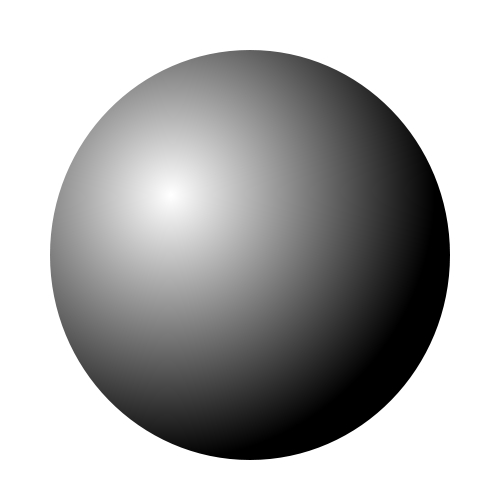
\includegraphics[width=.3\textwidth]{../figure/sphere.png}
\caption{Perfektiivinen aspekti rajattuna kokonaisuutena}
\end{figure}
\FloatBarrier

on imperfektiivinen aspekti enemmänkin kuin epämääräistä usvaa (ajatus
vertaukseen peräisin Nikunlassilta 2002: 176, joka puhuu \emph{kaasusta
tai nesteestä}):

\FloatBarrier
\begin{figure}[htbp]
\centering

\includegraphics[width=.6\textwidth]{../figure/silver-gray-mist-background.jpg}
\caption{Imperfektiivinen aspekti epämääräisenä, rajaamattomana ilmiönä}
\end{figure}
\FloatBarrier

On kuitenkin pidettävä mielessä, että aspektin kategoria on
monimutkainen ja monitahoinen ilmiö, jota ei ole mahdollista tai
järkevääkään yrittää puristaa yhteen virkkeeseen tai yhteen
ominaisuuteen. Ajatus sisäisestä rajasta lienee kuitenkin toimivampi
kuin tavallisessa kouluopetuksessa usein esitettävä \emph{toiminnan
suorittaminen loppuun vs.~toiminnan keskeneräisyys}. Ajattele vaikka
seuraavaa esimerkkilausetta:

\begin{enumerate}
\def\labelenumi{(\arabic{enumi})}
\tightlist
\item
  Ковальчук о чем-то \emph{пошутил} и басисто \emph{засмеялся}
\end{enumerate}

Kumpaakaan esimerkin 1 (perfektiivisistä) verbeistä ei erityisen hyvin
kuvaa ajatus siitä, että puhuja korostaisi niiden suorittamista loppuun.
\emph{Засмеятся}-verbi merkitsee \emph{nauramisen alkamista}, jolloin
ajatus rajasta ja toiminnasta kokonaisuutena tuntuu selvästi
järkevämmältä; \emph{пошутить} puolestaan merkitsee `vitsailemista
pikkaisen / vähän aikaa', ja loppuun suorittaminen vaikuttaa myös tässä
jonkin verran kömpelöltä tavalta ilmaista perfektiivisen aspektin
luonnetta.

Ajatus sisäisestä rajasta on kuitenkin sekin vielä sinänsä turhan
pelkistävä. Tähän liittyen Bondarko (2005: 230--231) esittää, että
kumpaakin aspektia on hedelmällistä tarkastella kokonaisen piirrejoukon
valossa, ja vertailla, mitä piirrettä mikin aspekti ilmentää usein, mitä
harvoin ja mitä ei lainkaan. Bondarkon esittämiä piirteitä ovat muun
muassa seuraavat:

\begin{itemize}
\tightlist
\item
  Toiminnan käsittäminen kokonaisuutena (sisäinen raja)
\item
  Prosessuaalisuus
\item
  Kesto
\item
  Toiminnan äkillinen alkaminen
\item
  Toiminnan samanaikaisuus ja peräkkäisyys
\end{itemize}

Prosessuaalisuus on esimerkiksi imperfektiiviselle aspektille
tyypillistä, sisäinen raja puolestaan perfektiiviselle. Kestoa aspektit
ilmaisevat kumpikin, mutta eri tavoin, äkillistä alkamista,
samanaikaisuutta ja peräkkäisyyttä myös, mutta erilaisin painotuksin.

\subsection{Aspektiparin käsite}\label{aspektiparin-kuxe4site}

Aspektien välinen oppositio toteutuu sanatasolla siten, että verbeistä
on tapana muodostaa aspektikategorian suhteen pareja. Voidaan
esimerkiksi ajatella, että verbit открыть ja открывать ovat oppositiossa
keskenään, niin että открыть ilmaisee perfektiivisyyttä, открывать
imperfektiivisyyttä. Aina ei kuitenkaan ole yksinkertaista määritellä,
mitkä osapuolet mihinkin pariin kuuluvat. Mikä olisi mielestäsi
aspektipari esimerkiksi niinkin tavallisen verbin kuin ехать
aspektipari? Поехать? Доехать? Приехать?

Edellisessä esimerkissä -- ja yleisemmälläkin tasolla -- aspektiparin
määrittämisestä tekee vaikeaa se, että kukin ehdotetuista pareista tuo
jotakin lisää verbin merkitykseen. Ехать-verbin tapauksessa verbiin
liittyy ehdotetusta parista riippuen mielikuva joko lähtemisestä,
saapumisesta, loppuun asti kulkemisesta tai muusta vastaavasta. Yleinen
aspektiparin määritelmä nimittäin kuuluu, että aspektiparin
\emph{muodostavat verbit, jotka ovat merkitykseltään täysin samoja,
mutta eroavat toisistaan aspektikategorian osalta}. Kuten Nikunlassi
(2002: 177) huomauttaa, on kuitenkin hankala määritellä, mikä
merkityksessä lopulta on aspektikategorian mukanaan tuomaa, mikä
leksikaalista eli sanan oman merkityksen piiriin kuuluvaa.

Aspektiparin määrittelyvaikeuksiin ei mennä tässä yhteydessä sen
syvemmälle. On kuitenkin hyvä muistaa, että verbit voivat muodostaa
selkeämpiä ja vähemmän selkeitä aspektipareja. Kaikkein selkeimmät
aspektiparit syntyvät silloin, kun perfektiivisestä verbistä
muodostetaan imperfektiivinen verbi suffiksin avulla:

\begin{itemize}
\tightlist
\item
  перечит/а/ть -- перечит/ыва/ть
\item
  рассмотр/е/ть -- рассматр/ива/ть
\item
  замет/и/ть -- замеч/а/ть
\end{itemize}

Prosessia, jossa perfektiivisestä aspektista muodostetaan
imperfektiivisen aspektin verbi suffiksin avulla, kutsutaan
\emph{imperfektivaatioksi} (имперфективация). Kun sananmuodostus
tapahtuu toiseen suuntaan -- kuten edellä ехать-esimerkissä -- syntyy
usein vähemmän selviä aspektipareja. Sananmuodostusta suuntaan
imperfektiivinen--perfektiivinen kutsutaan \emph{perfektivaatioksi}
(перфективация) ja se tapahtuu aina \emph{prefiksien} avulla:

\begin{itemize}
\tightlist
\item
  звонить -- позвонить
\item
  видеть -- увидеть
\item
  рисовать -- нарисовать
\item
  благодарить -- поблагодарить
\end{itemize}

Kuten edellä mainittiin, perfektivaation tuloksena on joskus verbejä,
joilla merkitys muuttuu selvästikin. Aina prefiksin lisäämistä
imperfektiiviseen verbiin ei voi lainkaan ajatella aspektiparin
tuottamisena. Ajattele vaikkapa imperfektiivistä играть-verbiä ja
perfektiivisiä verbejä \emph{выиграть} ja \emph{проиграть}.

Perfektivaatiossa käytettävien prefiksien määrä on suuri: mahdollisia
ovat esimerkiksi до, от, по, с, из, об, пере, про, с ja monet muut.
Imperfektivaatiossa käytettävien suffiksien määrä on rajatumpi.
Nikunlassin (2002: 166) luettelee muun muassa seuraavat:

\begin{itemize}
\tightlist
\item
  ива (прочитать -- прочитывать)
\item
  ева (заболеть -- заболевать)
\item
  а (обучить -- обучать, толкнуть -- толкать)
\end{itemize}

\subsection{Aspektin valinnasta}\label{aspektin-valinnasta}

Olen edellä jättänyt tarkoituksellisen vähälle huomiolle
sananmuodostuksellisen puolen aspektista. Tarkoitukseni on tällä
kurssilla keskittyä enemmän aspektiin funktionaalisen morfologian
kannalta ja pohtia, joskin vain pintapuolisesti ja melko nopeasti, ennen
kaikkea kysymystä siitä, milloin mitäkin aspektia tulisi tai kannattaisi
käyttää. Tähän kysymykseen paneudutaan seuraavilla kahdella luennolla.
Pohjustuksena niille on kuitenkin hyvä käydä läpi seuraavat huomiot.

\begin{enumerate}
\def\labelenumi{\arabic{enumi}.}
\tightlist
\item
  Jommankumman aspektin käyttäminen on harvoin normatiivisessa mielessä
  oikein tai väärin. Kyse on aina puhujan viestintätavoitteesta: usein
  molempi aspekti on \emph{mahdollinen}, mutta niillä on eri
  merkitykset.
\item
  Aspektin valintaan vaikuttavat monet puhtaan kieliopilliset tekijät.
  Kun pohdit aspektin käyttöä, mieti ainakin seuraavia seikkoja:

  \begin{itemize}
  \tightlist
  \item
    Mikä aikamuoto on kyseessä?
  \item
    Onko kyseessä kielto- vai myöntölause?
  \item
    Onko kyse indikatiivimuodoista vai kenties infinitiivistä?
  \item
    Edustaako tilanteessa käytettävä verbi jotakin \emph{teonlaatua}
    (tähän käsitteeseen pureudutaan luennolla 17)?
  \end{itemize}
\item
  Kuten jo todettua, aspektin merkitystä pohdittaessa ei kannata olla
  liian yksipuolinen vaan muistaa, että kyse on monitahoisista
  ilmiöistä. Kummastakin aspektista voidaan erottaa useita erilaisia
  merkityksiä. Voidaan ensinnäkin puhua imperfektiivisen ja
  perfektiivisen aspektin \emph{perusmerkityksistä} eli
  \emph{invarianteista merkityksistä} (общие видовые значения), jotka
  kuvaavat kaikkein tyyypillisintä tapaa käyttää kumpaakin aspektia.
  Näiden lisäksi voidaan eritellä tarkempia konteksteja ja
  käyttötilanteita, joissa kumpaakin aspektia käytetään jollain
  perusmerkityksestä mahdollisesti poikkeavalla tavalla. Tällaisissa
  tapauksissa puhutaan aspektin \emph{erityismerkityksistä} (частные
  видовые значения).
\end{enumerate}

\hyperdef{}{ref-bondarko2005}{\label{ref-bondarko2005}}
Bondarko, A.V. 2005. \emph{Теория Морфологических Категории И
Аспектологические Исследования}. Moskova: Jazyki slavjanskoj kultury.

\hyperdef{}{ref-klein1999}{\label{ref-klein1999}}
Klein, Wolfgang. (1994) 1999. \emph{Time in Language}. London:
Routledge.

\hyperdef{}{ref-nikunl}{\label{ref-nikunl}}
Nikunlassi, Ahti. 2002. \emph{Johdatus Venäjän Kieleen Ja Sen
Tutkimukseen}. Helsinki: Finn Lectura.

\end{document}
